\documentclass[11pt,letterpaper]{article}

% ─── Packages ─────────────────────────────────────────────────────────────────
\usepackage[margin=1in]{geometry}
\usepackage{graphicx}
\usepackage{xcolor}
\usepackage{tikz}
\usetikzlibrary{shapes.geometric, arrows.meta, positioning, fit, calc, backgrounds}
\usepackage{booktabs}
\usepackage{enumitem}
\usepackage{fancyhdr}
\usepackage{hyperref}
\usepackage{tcolorbox}
\usepackage{fontenc}
\usepackage{sectsty}
\usepackage{tabularx}
\usepackage{array}

% ─── Colors ───────────────────────────────────────────────────────────────────
\definecolor{milgreen}{HTML}{2D5016}
\definecolor{milgold}{HTML}{C5A300}
\definecolor{safebox}{HTML}{E8F5E9}
\definecolor{warnbox}{HTML}{FFF3E0}
\definecolor{infoblue}{HTML}{E3F2FD}
\definecolor{dangerred}{HTML}{FFEBEE}
\definecolor{stripred}{HTML}{D32F2F}
\definecolor{tokenblue}{HTML}{1565C0}
\definecolor{safegreen}{HTML}{2E7D32}
\definecolor{lightgray}{HTML}{F5F5F5}

% ─── Header / Footer ─────────────────────────────────────────────────────────
\pagestyle{fancy}
\fancyhf{}
\fancyhead[L]{\small\color{milgreen}\textbf{MLI Weekly Hours --- Security Report}}
\fancyhead[R]{\small\color{gray}UNCLASSIFIED // FOUO}
\fancyfoot[C]{\small\thepage}
\fancyfoot[R]{\small\color{gray}March 2026}
\renewcommand{\headrulewidth}{0.4pt}

% ─── Section styling ─────────────────────────────────────────────────────────
\sectionfont{\color{milgreen}}
\subsectionfont{\color{milgreen!80!black}}

% ─── tcolorbox styles ────────────────────────────────────────────────────────
\tcbset{
  safestyle/.style={colback=safebox, colframe=safegreen, fonttitle=\bfseries, left=6pt, right=6pt, top=4pt, bottom=4pt, boxrule=0.8pt},
  warnstyle/.style={colback=warnbox, colframe=orange!70!black, fonttitle=\bfseries, left=6pt, right=6pt, top=4pt, bottom=4pt, boxrule=0.8pt},
  infostyle/.style={colback=infoblue, colframe=blue!50!black, fonttitle=\bfseries, left=6pt, right=6pt, top=4pt, bottom=4pt, boxrule=0.8pt},
  dangerstyle/.style={colback=dangerred, colframe=red!70!black, fonttitle=\bfseries, left=6pt, right=6pt, top=4pt, bottom=4pt, boxrule=0.8pt}
}

\hypersetup{
  colorlinks=true,
  linkcolor=milgreen,
  urlcolor=tokenblue,
  pdftitle={MLI Weekly Hours - Data Privacy and Security Report},
  pdfauthor={DLIFLC Arabic School}
}

% ─── Document ─────────────────────────────────────────────────────────────────
\begin{document}

% ─── Title ────────────────────────────────────────────────────────────────────
\begin{center}
  {\color{milgreen}\rule{\textwidth}{2pt}}\\[12pt]
  {\Huge\bfseries\color{milgreen} Data Privacy \& Security Report}\\[8pt]
  {\Large MLI Weekly Hours Application}\\[6pt]
  {\large Defense Language Institute Foreign Language Center}\\
  {\large Arabic School}\\[8pt]
  {\color{milgreen}\rule{\textwidth}{2pt}}\\[10pt]
  {\large Version 1.0 \quad---\quad March 2026}\\[4pt]
  {\small UNCLASSIFIED // FOR OFFICIAL USE ONLY}
\end{center}

\vspace{16pt}

% ─── Executive Summary ───────────────────────────────────────────────────────
\section{Executive Summary}

The MLI Weekly Hours application processes instructor work-hour data to auto-fill DLIFLC reporting forms. Because this data contains \textbf{Personally Identifiable Information (PII)}---including instructor names, team assignments, and duty schedules---the application implements a multi-layer privacy architecture that ensures \textbf{no real names or sensitive data ever leave the user's browser}.

\begin{tcolorbox}[safestyle, title={Bottom Line Up Front}]
\begin{itemize}[nosep,leftmargin=*]
  \item All AI processing uses \textbf{anonymous tokens} (MLI\_1, MLI\_2), never real names
  \item Excel data is \textbf{stripped of all non-essential columns} before AI transmission
  \item The name-to-token mapping exists \textbf{only in browser memory}---never stored, never transmitted
  \item Free-text chat input is \textbf{automatically scrubbed} for known names
  \item No server, no database, no cookies---\textbf{fully client-side architecture}
\end{itemize}
\end{tcolorbox}

\vspace{10pt}

% ─── Architecture Overview ───────────────────────────────────────────────────
\section{System Architecture}

\subsection{Client-Side Only Design}

The application runs entirely in the user's web browser. There is no backend server, no database, and no persistent storage of any kind.

\begin{center}
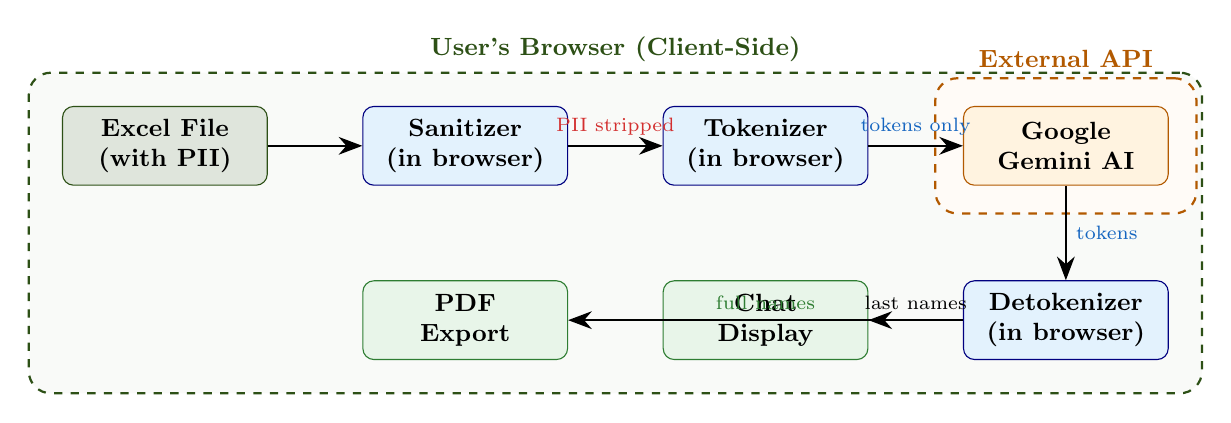
\begin{tikzpicture}[
  node distance=0.8cm and 1.2cm,
  box/.style={draw, rounded corners=4pt, minimum width=2.6cm, minimum height=1cm, align=center, font=\small\bfseries},
  userbox/.style={box, fill=milgreen!15, draw=milgreen},
  procbox/.style={box, fill=infoblue, draw=blue!50!black},
  aibox/.style={box, fill=warnbox, draw=orange!70!black},
  outbox/.style={box, fill=safebox, draw=safegreen},
  arr/.style={-{Stealth[length=3mm]}, thick},
  darr/.style={-{Stealth[length=3mm]}, thick, dashed, gray},
]

  % Nodes
  \node[userbox] (excel) {Excel File\\(with PII)};
  \node[procbox, right=of excel] (sanitize) {Sanitizer\\(in browser)};
  \node[procbox, right=of sanitize] (tokenize) {Tokenizer\\(in browser)};
  \node[aibox, right=of tokenize] (gemini) {Google\\Gemini AI};
  \node[procbox, below=1.2cm of gemini] (detokenize) {Detokenizer\\(in browser)};
  \node[outbox, left=of detokenize] (display) {Chat\\Display};
  \node[outbox, left=of display] (pdf) {PDF\\Export};

  % Arrows
  \draw[arr] (excel) -- (sanitize);
  \draw[arr] (sanitize) -- node[above, font=\scriptsize\color{stripred}] {PII stripped} (tokenize);
  \draw[arr] (tokenize) -- node[above, font=\scriptsize\color{tokenblue}] {tokens only} (gemini);
  \draw[arr] (gemini) -- node[right, font=\scriptsize\color{tokenblue}] {tokens} (detokenize);
  \draw[arr] (detokenize) -- node[above, font=\scriptsize] {last names} (display);
  \draw[arr] (detokenize) -- node[above, font=\scriptsize\color{safegreen}] {full names} (pdf);

  % Browser boundary
  \begin{scope}[on background layer]
    \node[draw=milgreen, dashed, thick, rounded corners=8pt, fill=milgreen!3,
          fit=(excel)(sanitize)(tokenize)(detokenize)(display)(pdf),
          inner sep=12pt, label={[font=\small\bfseries\color{milgreen}]above:User's Browser (Client-Side)}] {};
  \end{scope}

  % External boundary
  \begin{scope}[on background layer]
    \node[draw=orange!70!black, dashed, thick, rounded corners=8pt, fill=orange!3,
          fit=(gemini),
          inner sep=10pt, label={[font=\small\bfseries\color{orange!70!black}]above:External API}] {};
  \end{scope}

\end{tikzpicture}
\end{center}

\subsection{Technology Stack}

\begin{table}[h]
\centering
\begin{tabularx}{\textwidth}{lXl}
\toprule
\textbf{Component} & \textbf{Purpose} & \textbf{Data Exposure} \\
\midrule
React 18 (CDN) & UI rendering & None \\
Firebase Auth & Google Sign-In & Email only \\
Firebase AI Logic & Gemini 2.5 Flash proxy & Tokenized data only \\
SheetJS (XLSX) & Excel parsing & Client-side only \\
pdf-lib & PDF form filling & Client-side only \\
JSZip & Batch ZIP generation & Client-side only \\
\bottomrule
\end{tabularx}
\end{table}

% ─── PII Data Flow ───────────────────────────────────────────────────────────
\section{PII Protection: Detailed Data Flow}

\subsection{Stage 1: Excel Column Stripping}

When an Excel file is uploaded, the \texttt{sanitizeExcel()} function immediately strips it down to only the columns needed for hour classification.

\begin{center}
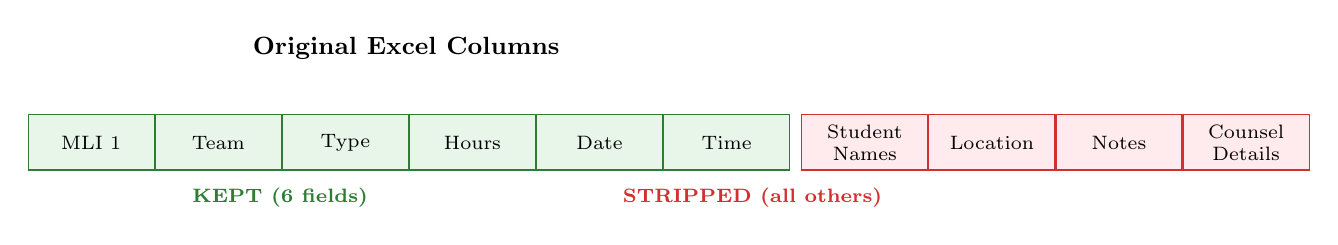
\begin{tikzpicture}[
  col/.style={draw, minimum width=1.6cm, minimum height=0.7cm, font=\scriptsize, align=center},
  kept/.style={col, fill=safebox, draw=safegreen},
  stripped/.style={col, fill=dangerred, draw=stripred},
]
  % Header
  \node[font=\small\bfseries] at (0, 1.2) {Original Excel Columns};

  % Kept columns
  \node[kept] (c1) at (-4, 0) {MLI 1};
  \node[kept, right=0pt of c1] (c2) {Team};
  \node[kept, right=0pt of c2] (c3) {Type};
  \node[kept, right=0pt of c3] (c4) {Hours};
  \node[kept, right=0pt of c4] (c5) {Date};
  \node[kept, right=0pt of c5] (c6) {Time};

  % Stripped columns
  \node[stripped, right=4pt of c6] (s1) {Student\\Names};
  \node[stripped, right=0pt of s1] (s2) {Location};
  \node[stripped, right=0pt of s2] (s3) {Notes};
  \node[stripped, right=0pt of s3] (s4) {Counsel\\Details};

  % Labels
  \node[font=\scriptsize\bfseries\color{safegreen}] at (-1.6, -0.7) {KEPT (6 fields)};
  \node[font=\scriptsize\bfseries\color{stripred}] at (4.4, -0.7) {STRIPPED (all others)};

\end{tikzpicture}
\end{center}

\begin{tcolorbox}[dangerstyle, title={What Gets Removed}]
\begin{itemize}[nosep,leftmargin=*]
  \item Student names (full names, nicknames, student IDs)
  \item Physical locations and room numbers
  \item Counseling details and behavioral notes
  \item Free-text comments and annotations
  \item Any column not explicitly: MLI, Team, Type, Hours, Date, Time
\end{itemize}
\end{tcolorbox}

\subsection{Stage 2: Name Tokenization}

Even the 6 kept fields undergo further anonymization. The MLI name column is replaced with anonymous tokens.

\begin{center}
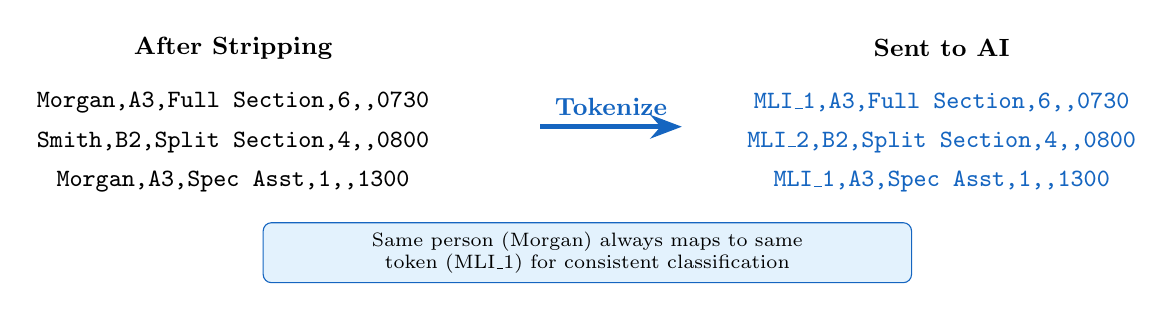
\begin{tikzpicture}[
  node distance=0.3cm,
  row/.style={font=\small\ttfamily},
]
  % Before
  \node[font=\small\bfseries] at (-3.5, 2) {After Stripping};
  \node[row] at (-3.5, 1.3) {Morgan,A3,Full Section,6,,0730};
  \node[row] at (-3.5, 0.8) {Smith,B2,Split Section,4,,0800};
  \node[row] at (-3.5, 0.3) {Morgan,A3,Spec Asst,1,,1300};

  % Arrow
  \draw[-{Stealth[length=4mm]}, ultra thick, color=tokenblue] (0.4, 1) -- node[above, font=\small\bfseries\color{tokenblue}] {Tokenize} (2.2, 1);

  % After
  \node[font=\small\bfseries] at (5.5, 2) {Sent to AI};
  \node[row, color=tokenblue] at (5.5, 1.3) {MLI\_1,A3,Full Section,6,,0730};
  \node[row, color=tokenblue] at (5.5, 0.8) {MLI\_2,B2,Split Section,4,,0800};
  \node[row, color=tokenblue] at (5.5, 0.3) {MLI\_1,A3,Spec Asst,1,,1300};

  % Note
  \node[draw=tokenblue, fill=infoblue, rounded corners=3pt, font=\scriptsize, text width=8cm, align=center] at (1, -0.6)
    {Same person (Morgan) always maps to same token (MLI\_1) for consistent classification};

\end{tikzpicture}
\end{center}

\subsubsection{Token Mapping (Browser Memory Only)}

\begin{center}
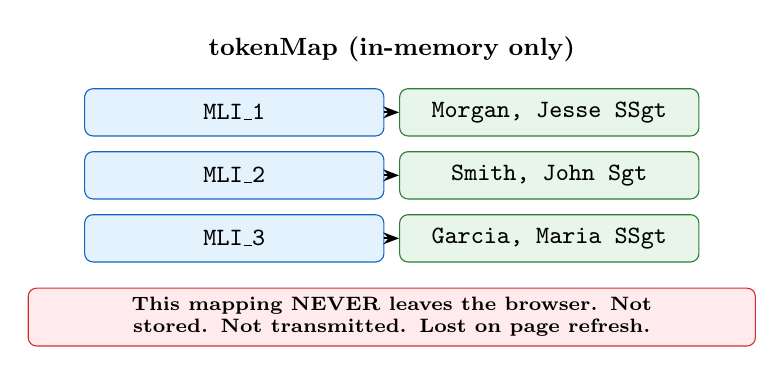
\begin{tikzpicture}[
  mapbox/.style={draw, rounded corners=3pt, minimum width=3.8cm, minimum height=0.6cm, font=\small\ttfamily, align=center},
  tok/.style={mapbox, fill=infoblue, draw=tokenblue},
  namebox/.style={mapbox, fill=safebox, draw=safegreen},
  arr/.style={-{Stealth[length=2mm]}, thick},
]
  \node[font=\small\bfseries] at (0, 2.2) {tokenMap (in-memory only)};

  \node[tok] (t1) at (-2, 1.4) {MLI\_1};
  \node[namebox] (n1) at (2, 1.4) {Morgan, Jesse SSgt};
  \draw[arr] (t1) -- (n1);

  \node[tok] (t2) at (-2, 0.6) {MLI\_2};
  \node[namebox] (n2) at (2, 0.6) {Smith, John Sgt};
  \draw[arr] (t2) -- (n2);

  \node[tok] (t3) at (-2, -0.2) {MLI\_3};
  \node[namebox] (n3) at (2, -0.2) {Garcia, Maria SSgt};
  \draw[arr] (t3) -- (n3);

  \node[draw=stripred, fill=dangerred, rounded corners=3pt, font=\scriptsize\bfseries, text width=9cm, align=center] at (0, -1.2)
    {This mapping NEVER leaves the browser. Not stored. Not transmitted. Lost on page refresh.};

\end{tikzpicture}
\end{center}

\subsection{Stage 3: Free-Text Scrubbing}

When a user types a message in the chat (e.g., \textit{``Morgan taught A3 full section 15 hours''}), the application automatically scans for known names from any previously uploaded Excel and replaces them with tokens before transmission.

\begin{center}
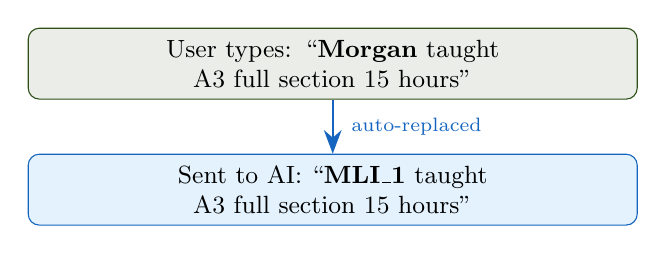
\begin{tikzpicture}[
  msg/.style={draw, rounded corners=4pt, minimum height=0.9cm, font=\small, align=center, text width=7.5cm},
]
  \node[msg, fill=milgreen!10, draw=milgreen] (before) at (0, 1)
    {User types: ``\textbf{Morgan} taught A3 full section 15 hours''};
  \node[msg, fill=infoblue, draw=tokenblue] (after) at (0, -0.6)
    {Sent to AI: ``\textbf{MLI\_1} taught A3 full section 15 hours''};
  \draw[-{Stealth[length=3mm]}, thick, color=tokenblue] (before) -- node[right, font=\scriptsize\color{tokenblue}, xshift=3pt] {auto-replaced} (after);
\end{tikzpicture}
\end{center}

\begin{tcolorbox}[infostyle, title={How Free-Text Scrubbing Works}]
\begin{enumerate}[nosep,leftmargin=*]
  \item On Excel upload, the app builds a \texttt{nameToToken} lookup (e.g., MORGAN $\rightarrow$ MLI\_1)
  \item Before \textit{every} message sent to the AI, the text is scanned against this lookup
  \item Matches are case-insensitive with word-boundary detection to avoid false positives
  \item If no Excel has been uploaded yet, there are no names to scrub (acceptable---see Section~\ref{sec:residual})
\end{enumerate}
\end{tcolorbox}

\subsection{Stage 4: Response Detokenization}

When the AI responds using tokens, the application translates them back to readable names \textbf{entirely client-side} before displaying to the user.

\begin{center}
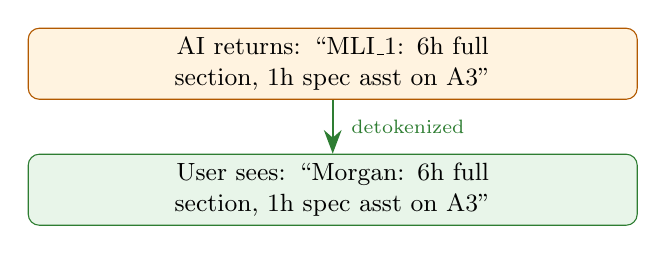
\begin{tikzpicture}[
  msg/.style={draw, rounded corners=4pt, minimum height=0.9cm, font=\small, align=center, text width=7.5cm},
]
  \node[msg, fill=warnbox, draw=orange!70!black] (ai) at (0, 1)
    {AI returns: ``MLI\_1: 6h full section, 1h spec asst on A3''};
  \node[msg, fill=safebox, draw=safegreen] (user) at (0, -0.6)
    {User sees: ``Morgan: 6h full section, 1h spec asst on A3''};
  \draw[-{Stealth[length=3mm]}, thick, color=safegreen] (ai) -- node[right, font=\scriptsize\color{safegreen}, xshift=3pt] {detokenized} (user);
\end{tikzpicture}
\end{center}

\subsection{Stage 5: PDF Export with Full Names}

When generating the final PDF, tokens are expanded to full names using the browser-only mapping. The full name (e.g., ``Morgan, Jesse SSgt'') is written into the PDF \texttt{Name} field. This expansion happens entirely in the browser---the full name is never sent to any external service.

% ─── What Google Sees ────────────────────────────────────────────────────────
\section{What Google's AI Actually Receives}

\begin{tcolorbox}[warnstyle, title={Exact Data Sent to Gemini 2.5 Flash}]
\begin{verbatim}
MLI,Team,Type,Hours,Date,Time
MLI_1,A3,Full Section (6 hours),6,Mon,0730
MLI_1,A3,Spec Asst (1 hours),1,Mon,1300
MLI_2,B2,Split Section (4 hours),4,Tue,0800
MLI_1+MLI_3,A3,Full Section (6 hours),6,Wed,0730
MLI_2,B2,Class Prep (2 hours),2,Thu,
\end{verbatim}
\end{tcolorbox}

\begin{tcolorbox}[safestyle, title={What Google Does NOT Receive}]
\begin{itemize}[nosep,leftmargin=*]
  \item Real names (first, last, full, rank)
  \item Student names or identifiers
  \item Locations, room numbers, building names
  \item Counseling narratives or behavioral notes
  \item The token-to-name mapping
  \item Any data from columns beyond the 6 extracted fields
\end{itemize}
\end{tcolorbox}

% ─── Google's Data Policy ────────────────────────────────────────────────────
\section{Google AI Data Governance}

The application uses \textbf{Firebase AI Logic} to proxy requests to Google's Gemini API. Per Google's published policies:

\begin{table}[h]
\centering
\begin{tabularx}{\textwidth}{lX}
\toprule
\textbf{Policy} & \textbf{Detail} \\
\midrule
Training data & API inputs are \textbf{not used} to train Google's models \\
Data retention & Inputs may be temporarily processed but are \textbf{not stored long-term} \\
Logging & Google may log requests for abuse monitoring (tokenized data only) \\
Encryption & All data in transit is encrypted via \textbf{TLS 1.3} \\
Region & Processed on Google Cloud infrastructure \\
\bottomrule
\end{tabularx}
\caption{Google Gemini API data handling (source: Google AI Terms of Service)}
\end{table}

\begin{tcolorbox}[infostyle, title={Defense in Depth}]
Even if Google were to retain or inspect the data, they would see only anonymous tokens (MLI\_1, MLI\_2), team designations (A3, B2), and hour categories. There is \textbf{no way to reconstruct real identities} from this data alone.
\end{tcolorbox}

% ─── Threat Model ────────────────────────────────────────────────────────────
\section{Threat Model}

\begin{table}[h]
\centering
\begin{tabularx}{\textwidth}{lXll}
\toprule
\textbf{Threat} & \textbf{Description} & \textbf{Mitigated?} & \textbf{How} \\
\midrule
Name leakage to AI & Real names sent to Gemini & Yes & Tokenization \\
Column leakage & Student data sent to AI & Yes & Column stripping \\
Free-text leakage & User types names in chat & Partial$^*$ & Auto-scrubbing \\
Network interception & Man-in-the-middle attack & Yes & TLS encryption \\
Data at rest & PII stored on disk/server & Yes & No storage at all \\
Browser extension & Malicious extension reads DOM & N/A & Outside app scope \\
Session persistence & PII survives page close & Yes & All state in memory \\
PDF contains PII & Exported PDF has real names & By design & User's local file \\
\bottomrule
\end{tabularx}
\caption{Threat assessment matrix}
\end{table}

\label{sec:residual}
$^*$\textit{Free-text scrubbing only works for names known from a prior Excel upload. If a user types a name before uploading any Excel file, it will pass through unscrubbed. A notice in the chat UI reminds users that names are automatically anonymized.}

% ─── Data Lifecycle ──────────────────────────────────────────────────────────
\section{Data Lifecycle}

\begin{center}
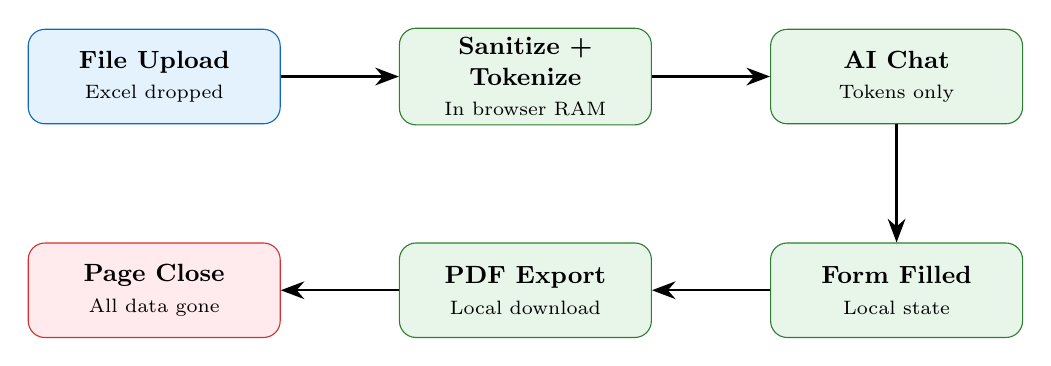
\begin{tikzpicture}[
  node distance=1.5cm,
  phase/.style={draw, rounded corners=6pt, minimum width=3.2cm, minimum height=1.2cm, align=center, font=\small\bfseries},
  create/.style={phase, fill=infoblue, draw=tokenblue},
  live/.style={phase, fill=safebox, draw=safegreen},
  destroy/.style={phase, fill=dangerred, draw=stripred},
  arr/.style={-{Stealth[length=3mm]}, thick},
]
  \node[create] (upload) {File Upload\\{\scriptsize\normalfont Excel dropped}};
  \node[live, right=of upload] (process) {Sanitize +\\Tokenize\\{\scriptsize\normalfont In browser RAM}};
  \node[live, right=of process] (ai) {AI Chat\\{\scriptsize\normalfont Tokens only}};
  \node[live, below=of ai] (result) {Form Filled\\{\scriptsize\normalfont Local state}};
  \node[live, left=of result] (pdf) {PDF Export\\{\scriptsize\normalfont Local download}};
  \node[destroy, left=of pdf] (gone) {Page Close\\{\scriptsize\normalfont All data gone}};

  \draw[arr] (upload) -- (process);
  \draw[arr] (process) -- (ai);
  \draw[arr] (ai) -- (result);
  \draw[arr] (result) -- (pdf);
  \draw[arr] (pdf) -- (gone);
\end{tikzpicture}
\end{center}

\begin{tcolorbox}[safestyle, title={No Persistence Guarantee}]
\begin{itemize}[nosep,leftmargin=*]
  \item \textbf{No cookies} store PII
  \item \textbf{No localStorage} is used for form data or names
  \item \textbf{No IndexedDB} stores any user information
  \item \textbf{No server} receives or retains the original Excel file
  \item Closing or refreshing the browser tab \textbf{destroys all data permanently}
\end{itemize}
\end{tcolorbox}

% ─── Compliance ──────────────────────────────────────────────────────────────
\section{Compliance Considerations}

\begin{table}[h]
\centering
\begin{tabularx}{\textwidth}{lX}
\toprule
\textbf{Standard} & \textbf{Relevance} \\
\midrule
DoD Privacy Act (5 U.S.C. \S552a) & PII is anonymized before external transmission; no PII is stored in any system of records \\
AR 25-2 / DoDI 8500.01 & Data in transit is encrypted (TLS); no data at rest; client-side only architecture \\
NIST SP 800-122 (PII Guide) & Tokenization is a recognized de-identification technique that removes direct identifiers \\
DLIFLC IT Policies & No data leaves the .mil/.gov network beyond anonymized hour classifications \\
\bottomrule
\end{tabularx}
\end{table}

% ─── Summary ─────────────────────────────────────────────────────────────────
\section{Summary of Protections}

\begin{center}
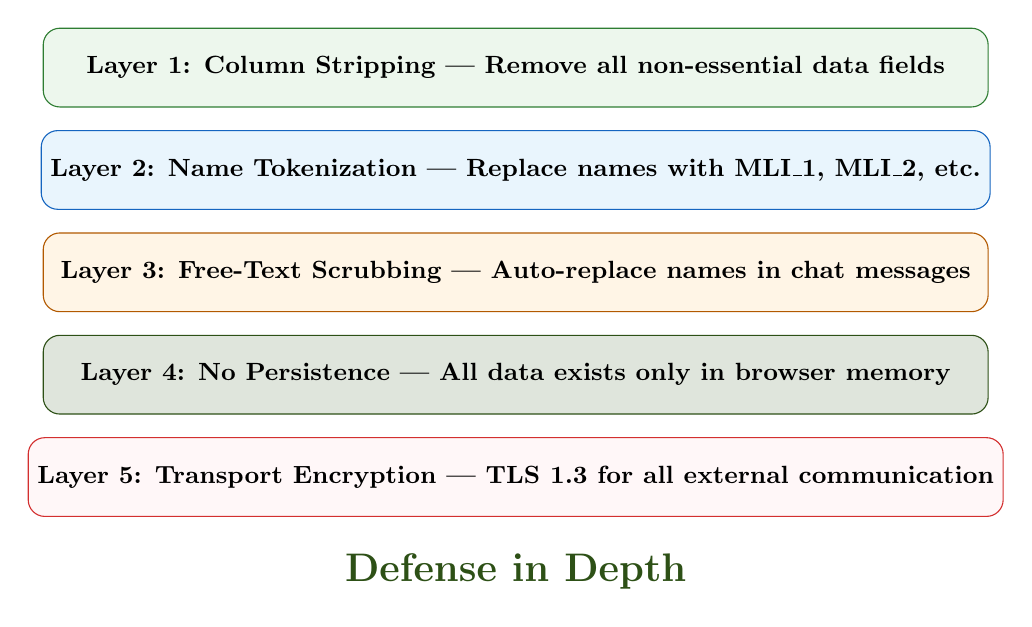
\begin{tikzpicture}[
  layer/.style={draw, rounded corners=6pt, minimum width=12cm, minimum height=1cm, align=center, font=\small\bfseries},
]
  \node[layer, fill=safebox!80, draw=safegreen] (l1) at (0, 4) {Layer 1: Column Stripping --- Remove all non-essential data fields};
  \node[layer, fill=infoblue!80, draw=tokenblue] (l2) at (0, 2.7) {Layer 2: Name Tokenization --- Replace names with MLI\_1, MLI\_2, etc.};
  \node[layer, fill=warnbox!80, draw=orange!70!black] (l3) at (0, 1.4) {Layer 3: Free-Text Scrubbing --- Auto-replace names in chat messages};
  \node[layer, fill=milgreen!15, draw=milgreen] (l4) at (0, 0.1) {Layer 4: No Persistence --- All data exists only in browser memory};
  \node[layer, fill=dangerred!40, draw=stripred] (l5) at (0, -1.2) {Layer 5: Transport Encryption --- TLS 1.3 for all external communication};

  \node[font=\Large\bfseries\color{milgreen}] at (0, -2.4) {Defense in Depth};
\end{tikzpicture}
\end{center}

\vspace{12pt}

\begin{tcolorbox}[safestyle, title={Conclusion}]
The MLI Weekly Hours application implements a \textbf{defense-in-depth} approach to PII protection. Through column stripping, name tokenization, free-text scrubbing, zero persistence, and transport encryption, the system ensures that \textbf{no personally identifiable information is ever transmitted to external services}. The only data that leaves the browser is anonymized hour-classification data that cannot be traced back to any individual without access to the user's active browser session.

\vspace{6pt}
\textbf{This application is safe for processing MLI work-hour data containing PII.}
\end{tcolorbox}

\vfill
\begin{center}
\small\color{gray}
Prepared for DLIFLC Arabic School\\
MLI Weekly Hours Application v1.0\\
\today
\end{center}

\end{document}
